\chapter{Numerical Computations of Bose-Hubbard Model}
For the numerical computations the \textit{density-matrix renormalization group} (DMRG) method is used. In this method a general state is represented as a product of matrices, otherwise known as a \textit{matrix product state} or MPS. This is achieved through a series of Schmidt decompositions, where in each iteration the eigenstates of the decomposition contributing the least to the state are truncated. Hence, matrix product states avoids the otherwise exponential growth of the Hilbert space with increasing particle number \cite{schollwock}.\\
Another important feature of matrix product states is how they follow an area law, meaning the scaling of entropy across the boundary of two regions of the system is linear \cite{Cramer}. Thus, in one dimension the entropy across a cut of the system is constant. This is essential for the success of the MPS representation, as one only has to consider a tiny portion of the full Hilbert space when performing a ground state search.\\
Hence, the DMRG algorithm, which iteratively performs ground state searches while sweeping over physical sites, is capable of accurately describing one dimensional many-body systems \cite{Kuhner2000, Kollath2004}. 


\section{Correlation Functions}
Examining the correlation functions of the Bose-Hubbard model is of special interest, since it relates to the interference pattern of particles measured when performing experiments \cite{Kashurnikov2002}, as well as the Superfluid-Mott Insulator phase transition \cite{Kuhner2000}.\\  
Although the MPS formalism excels at describing one dimensional systems, it struggles with describing the SF correlations, due to how it is constructed.
Consider an MPS of the form
\begin{equation}
	\ket{\psi} = \sum_{\{ j \} } \left( \prod_{n \in \mathbb{Z}} M^{j_n} \right) \ket{\{ j \}} \; ,
\end{equation}
where the $M$'s are the matrices of the MPS, and $j_n$ are the physical indices. The \textit{transfer operator} is defined as
\begin{equation}
	\hat{E}^{[n]} = \sum_{\alpha_{n-1}, \alpha_{n-1}'} \sum_{\alpha_{n}, \alpha_{n}'} \left( \sum_{j_n} M^{[n] j_n *} \otimes  M^{[n] j_n} \right)_{(\alpha_{n-1} \alpha_{n-1}'),(\alpha_{n}  \alpha_{n}')} \left( \ket{\alpha_{n-1}}\bra{\alpha_{n-1}'} \right) \left( \ket{\alpha_{n}}\bra{\alpha_{n}'} \right) \; ,
\end{equation}   
where the expression in the brackets is the matrix elements of the operator, and $\alpha_n$ are the physical indices of the matrices. The transfer operator is essentially a complete, positive map from operators defined on a block of the lattice of length $n-1$ to a block of length $n$, such that
\begin{equation}
	\{ \ket{\alpha_{n-1}}\bra{\alpha_{n-1}'} \} \to \{ \ket{\alpha_{n}}\bra{\alpha_{n}'} \} \; .
\end{equation}
One important property of the transfer operator, or transfer matrix, is that all eigenvalues $|\lambda_k| \leq 1 $ \cite{schollwock}. \\
Generalizing the transfer operator to contraction with an operator $\hat{O}$ gives
\begin{equation}
	E_{O}^{[n]} = \sum_{j_n , j_n '} O^{j_n , j_n '} M^{[n] j_n *} \otimes  M^{[n] j_n '} \; .
\end{equation}
Using this one can write the correlation function of two general operators on sites $i$ and $j$ as
\begin{align}
	\bra{\psi} \hat{O}^{[i]} \hat{O}^{[j]} \ket{\psi} &= \Tr E^{[1]} \ldots E^{[i-1]} E_{O}^{[i]} E^{[i+1]} \ldots E^{[j-1]} E_{O}^{[j]} E^{[j+1]} \ldots E^{[L]} \nonumber \\
	&= \Tr E_{O}^{[i]} E^{[j-i-1]} E_{O}^{[j]} E^{[L-j+i-1]} \nonumber \\ 
	&= \sum_{l , k} \bra{l} E_{O}^{[i]} \ket{k} \lambda_{k}^{j-i-1} \bra{k} E_{O}^{[j]} \ket{l} \lambda_{l}^{L-j+i-1} \nonumber \\ 
	&= \sum_{k} \bra{1} E_{O}^{[i]} \ket{k} \lambda_{k}^{j-i-1} \bra{k} E_{O}^{[j]} \ket{1} \quad (L \to \infty)
\end{align}
where $\lambda$ is the eigenvalues of the transfer matrix, and $L$ is the length of the system. Since $|\lambda_k| \leq 1 $, only the leading eigenvalue $\lambda_1 = 1$ remains as $L \to \infty$. Defining the distance between two sites as $r = |j - i -1|$ and the correlation decay, or correlation length, as $\xi_k = -1/\ln \lambda_k$, allows one to write the correlation function as
\begin{equation}
	\frac{\bra{\psi} \hat{O}^{[i]} \hat{O}^{[j]} \ket{\psi}}{\braket{\psi | \psi}} = c_1 + \sum_{k = 2} c_k e^{-r/ \xi_k} \; , \label{eq:corrfunction}
\end{equation}
where $c_k = \bra{1} E_{O}^{[i]} \ket{k} \bra{k} E_{O}^{[j]} \ket{1}$. \cite{schollwock} \\
Equation \ref{eq:corrfunction} shows that the correlation function is a linear combination of exponential functions. Since this was derived without any assumptions regarding neither the MPS nor the operators, this results can be considered general. Thus, any finite-dimensional MPS will only be able to approximate the true correlation of a system.\\
This is the cause of the difficulty of describing the Superfluid single-particle correlations. While single-particle correlations decay exponentially for the Mott-Insulator, it decays following a power-law for Superfluids
\begin{equation}
	\braket{\hat{a}_{i}^{\dag} \hat{a}_{j}} \sim |i - j|^{-K_b /2} \; ,
\end{equation}
where $K_b$ is the Tomonaga-Luttinger parameter \cite{characPhases}. For short distances equation \ref{eq:corrfunction} is able to accurately approximate a power-law, however, as distances grow larger, only the slowest exponential decay will survive. Hence, the correlation turns into a pure exponential decay with $\xi = -1/ \ln \lambda$, where $\lambda$ is the largest eigenvalue of $\hat{E}$ contributing to the correlation.

\subsection{Visualization of density matrices}
One way of displaying the correlations of the system is to plot its density matrix, whose entries are given by
\begin{equation}
	\rho_{i,j} = \bra{\psi} \hat{a}_{i}^{\dag} \hat{a}_j \ket{\psi} \; .
\end{equation}
\begin{figure}[h!]
    \centering
    \begin{subfigure}[t]{0.49\textwidth}
        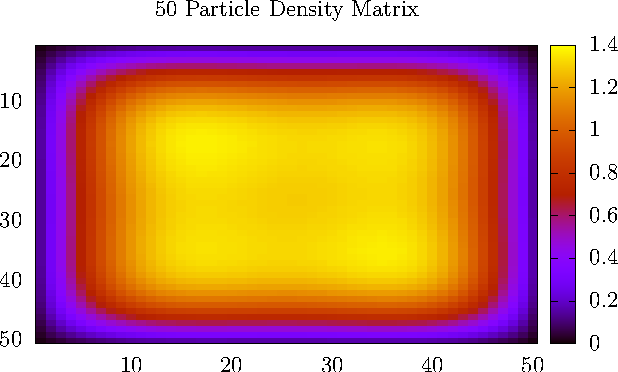
\includegraphics[width=\textwidth]{Figures/DensityMatSF30sweeps.pdf}
        \caption{\textit{Norm value of density matrix entries for $U/J = 0$.}}
        \label{fig:DensityMatSF}
    \end{subfigure}
    ~
    \begin{subfigure}[t]{0.49\textwidth}
        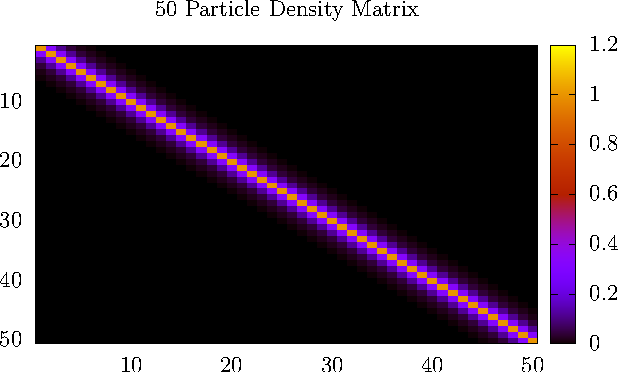
\includegraphics[width=\textwidth]{Figures/DensityMatMI.pdf}
        \caption{\textit{Norm value of density matrix entries for $U/J = 12$.}}
        \label{fig:DensityMatMI}
    \end{subfigure}
    ~
    \begin{subfigure}[t]{0.49\textwidth}
        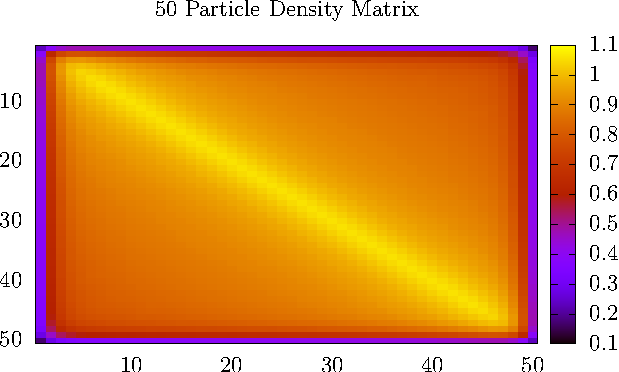
\includegraphics[width=\textwidth]{Figures/U050.pdf}
        \caption{\textit{Norm value of density matrix entries for $U/J = 0.5$.}}
        \label{fig:DensityMat05}
    \end{subfigure}
    ~
    \begin{subfigure}[t]{0.49\textwidth}
        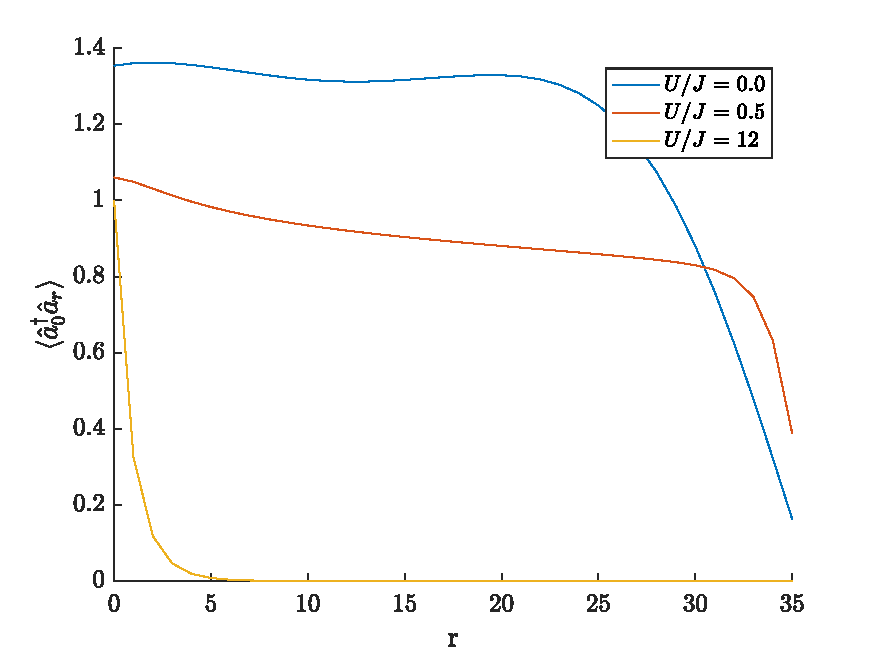
\includegraphics[width=0.9\textwidth]{Figures/correlationlength.pdf}
	\caption{\textit{Correlation function plotted as a function of distance from the diagonal element of the correlation matrix.}}
	\label{fig:expDecayCorrFunc}
    \end{subfigure}    
\end{figure}
Figures \ref{fig:DensityMatSF} and \ref{fig:DensityMatMI} show the density matrix of the 50 particle system plotted for the Superfluid and the Mott-Insulator limit respectively. In the SF limit long-range correlations are present, which is seen by large off-diagonal elements. However, as discussed previously, in the MPS approximation all correlations decay exponentially, which causes issues when trying to approximate the very long range correlations of the system. This is visualized in figure \ref{fig:expDecayCorrFunc} where the correlation function is plotted against distance from the diagonal. The Superfluid graph has a hump on it, which is an artifact of the DMRG algorithm. Due to the very long correlation length the graph should be almost flat except for the rapid drop in the end, which is due to the open boundary conditions. The graph in figure \ref{fig:expDecayCorrFunc} is the result of the DMRG algorithm attempting to express this long range correlation as a series of exponentials.\\
In the MI limit no interaction takes place between sites and the correlation length is zero,  leading to a correlation matrix consisting only of diagonal elements of equal magnitude. Figure \ref{eq:MI_lim} shows some off-diagonal elements of non-zero magnitude, however, this system is not a pure Mott-Insulator, as $U/J = 12$. Nevertheless, the correlations are well described by only a single exponential function, as shown in figure \ref{fig:expDecayCorrFunc}.\\
Finally, figure \ref{fig:DensityMat05} illustrates the density matrix for a system with $U/J = 0.5$, which is primarily as Superfluid, although, as seen in the figure, has a well defined diagonal. Inspecting its correlation function reveals that the best approximation is by a power-law, thus confirming that the system is indeed a Superfluid. 


\section{Condensate Fraction}

Recall the Bose-Hubbard Hamiltonian (equation \ref{BHhamil}), which supports the two distinct quantum phases: The Superfluid (SF) phase, $U/J \ll 1$, which exhibit long range correlations, and the Mott-Insulator (MI) phase, $U/J \gg 1$, where no interaction between neighboring sites is present. The SF phase is a Bose-Einstein condensate with special attributes, as it exhibits maximal de-localization of the particles and can be approximated as a coherent state. On the other hand, as the individual sites are completely decoupled in the MI phase, no condensate is present. \\
According to the Penrose-Onsager criterion, a Bose-Einstein condensate, and by extension the SF state, is present if and only if the largest eigenvalue, $\lambda_1$, of the single-particle density matrix, $\rho^{(1)}$, is macroscopic
\begin{equation}
	f_c = \frac{\lambda_1}{N_{\mathrm{particles}}} > 0 \; ,
\end{equation} 
where $f_c$ is the \textit{condensate fraction} and $N_{\mathrm{particles}}$ is the total number of particles \cite{PenroseOnsager}. Thus, the condensate fraction can be used to determine which state is the dominant of the system, as
\begin{align}
	\lim_{N_{\mathrm{particles}} \to \infty} f_{c}^{\mathrm{SF}} &\to 1 \label{eq:SF_lim} \\
	\lim_{N_{\mathrm{particles}} \to \infty} f_{c}^{\mathrm{MI}} &\to 0 \; , \label{eq:MI_lim}
\end{align}
where the filling-fraction $n = N_{\mathrm{particles}}/N_{\mathrm{sites}}$ is held constant. While the limit for the SF phase will be reached for any number of particles, the MI phase will only be reached in the limit $N_{\mathrm{particles}} \to \infty$.

\subsection{Calculated condensate fractions}
In order to test the precision of MPS formalism and the ITensor library, the condensate fraction was calculated for a series of $U/J$ with varying particle number. For this the library's implementation of the DMRG algorithm was used, where the number of sweeps was selected, such that the bond dimension remained the same when adding more sweeps. In this case 5 sweeps with a maximum bond dimension of 200 was sufficient. All calculations were performed with unit occupancy. These results were then compared to a similar calculation using exact diagonalisation.

\begin{figure}[h!]
    \centering
    \begin{subfigure}[t]{0.49\textwidth}
        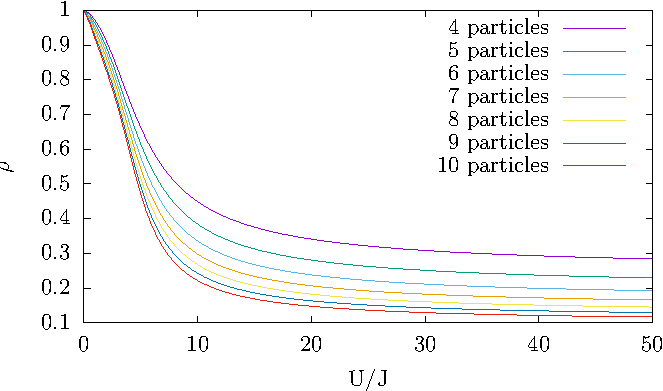
\includegraphics[width=\textwidth]{Figures/Condfrac_4to10.pdf}
        \caption{\textit{Condensate fraction calculated from an MPS after performing 5 DMRG sweeps.}}
        \label{fig:Condfrac_4to10}
    \end{subfigure}
    ~
    \begin{subfigure}[t]{0.49\textwidth}
        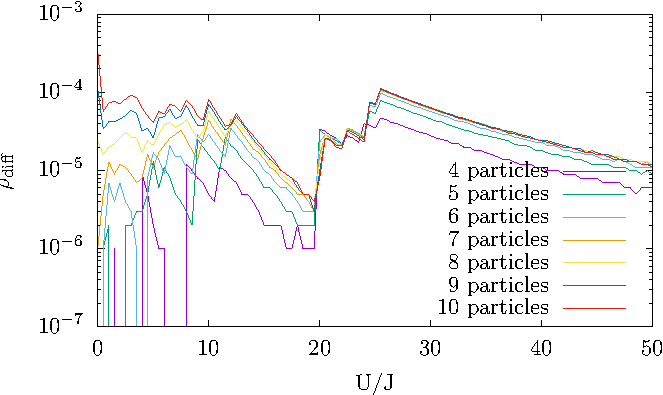
\includegraphics[width=\textwidth]{Figures/Confrac_exactvsMPS.pdf}
        \caption{\textit{Absolute difference between the condensate fraction calculated using MPS and using exact diagonalisation.}}
        \label{fig:Condfrac_exactvsMPS}
    \end{subfigure}    
\end{figure}
Figure \ref{fig:Condfrac_4to10} shows the condensate fraction for various $U/J$ calculated using MPS. In the limit $U/J = 0$ the condensate fraction is unit as expected, thus confirming that the system is indeed in the SF state. The condensate fraction never reaches zero, as this is only achieved in the thermodynamic limit as described by equation \ref{eq:MI_lim}. However, the condensate fraction does decrease with increasing particle number as would be expected.\\
In figure \ref{fig:Condfrac_exactvsMPS} the results of the MPS calculation is compared to exact diagonalisation by displaying the absolute difference between the two calculations. It is clear that the two approaches yield very similar results for low particle-number.\\
Attempting to use exact diagonalisation for large particle numbers is futile due to the exponential scaling of the Hilbert space, however, as mentioned, this is not an issue using matrix product states, since low contributing eigenstates are truncated. 
\begin{figure}[h!]
	\centering
	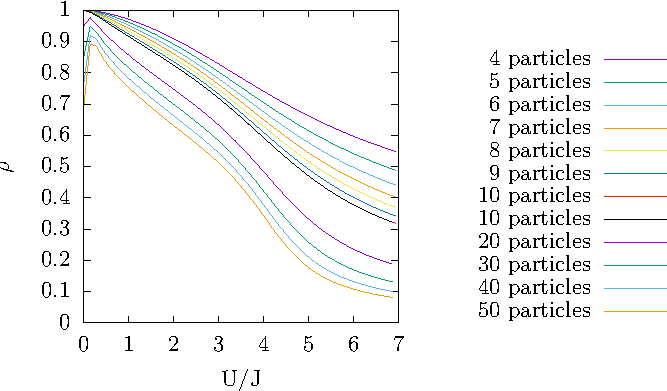
\includegraphics[width=0.9\textwidth]{Figures/Condfrac_4to50.pdf}
	\caption{\textit{Condensate fraction calculated from an MPS after performing 20 DMRG sweeps.}}
	\label{fig:Condfrac_4to50}
\end{figure}
Figure \ref{fig:Condfrac_4to50} shows the results of the DMRG calculations for up to 50 particles. The condensate fraction behaves as expected in the $U/J \gg 1$ limit, as it tends towards zero for larger particle numbers. Note, that in the SF limit the condensate fraction does not quite reach 1. However, this can be understood when considering figure \ref{fig:expDecayCorrFunc}, as the DMRG algorithm is unable to describe the very long ranged correlation of the Superfluid.
Smaller systems do not have this issue, as boundary effects has an influence on a much larger part of the system. Thus, these systems barely show any sign of long ranged correlations making them easy to approximate.\\
Some measures can be taken when using the DMRG algorithm in order to minimize errors. Accurately describing long range correlations requires multiple sweeps, as the algorithm iteratively has to approximate an almost constant function with a series of exponentials. Figure \ref{fig:sweepdependence} displays the condensate fraction in the Superfluid limit as a function of number of sweeps. Clearly, performing more sweeps yields a better result.
\begin{figure}[h!]
    \centering
    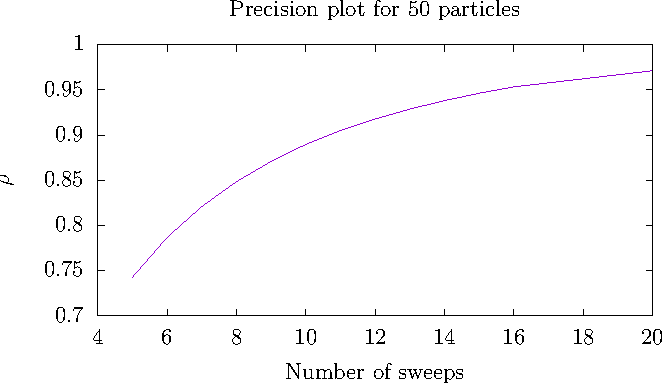
\includegraphics[width=0.9\textwidth]{Figures/condFracSweeps.pdf}
    \caption{\textit{SF condensate fraction as a function of number of sweeps of the DMRG algorithm. A max bond dimension of 250 was used.}}
    \label{fig:sweepdependence}
\end{figure}
Furthermore, one observes numerically, that increasing the maximal bond dimension $D$ results in a more accurate long-range representation of correlations. Thus, calculating correlation functions for various values of $D$ is a great way of estimating the convergence of the correlations for a given length scale \cite{schollwock}.\\

In \cite{Kuhner2000} the critical point of phase transition between the Superfluid and Mott-Insulator is determined as $\left( \frac{U}{J} \right)_{crit} = 3.37$. This is computed by determining the point at which the Luttinger liquid parameter is $K =  \frac{1}{2}$. Examining figure \ref{fig:Condfrac_4to50} one notices a hump on the graph in the vicinity of this critical ratio, however, no clear indication of a phase transition is present. In the thermodynamic limit one would expect the condensate fraction to drop to zero as the critical ratio is reached (as observed in 2D by \cite{Spielman2008}), although at 50 particles the condensate fraction is only around $0.5$. One could extrapolate data from several computations using different particle numbers in order to determine the location of the critical point. However, this would require computations using larger systems in order to minimize the boundary effects.\\  


\section{Time Evolution}
Recall the expression for the superfluid state
\begin{equation}\label{eq:SF_psi}
\lvert \psi \rangle = C \sum_{j=0}^{\infty} \frac{\alpha^j}{\sqrt{j!}}\lvert j\rangle,
\end{equation}
Recent experimental advances have made it possible to change the Hamiltonian almost instantaneously, allowing for a wide array of new experiments. In the current section, we will look at the case of an SF Hamiltonian,
\begin{equation}\label{eq:SF_ham}
\hat{H} = -J \sum_{\braket{i,j}} \hat{a}_{i}^{\dag} \hat{a}_j,
\end{equation}
 present long enough for the condensate to reach the ground state in eq. \ref{eq:SF_psi} suddenly being switched to a pure Mott Hamiltonian,
\begin{equation}
 \hat{H} = \frac{U}{2} \sum_{i} \hat{n}_i \left( \hat{n}_i -1 \right).
\end{equation}
%
In this case, the time evolution of the state can be described by
\begin{equation}
\lvert \psi (t) \rangle = C \sum_{j=0}^{\infty} \e^{-it \frac{U}{2} j(j-1)}\frac{\alpha^j}{\sqrt{j!}}\lvert j\rangle,
\end{equation}
and since $j(j-1)/2\in \mathbb{N}$ for all $j$, we will regain the superfluid state at times $p2\pi/U$,
\begin{equation}
\lvert \psi (p2\pi/U) \rangle = \lvert \psi (0) \rangle,
\end{equation}
for all integers $p$, whereby we should see a revival of the condensate fraction, as described in \ref{CondFrac}.\\

Further testing the applicability of the MPS formalism using ITensor library for time evolution, we evolved an SF state in time first with respect to a pure Mott Hamiltonian ($U=1$, $J=0$), then with respect to a slightly different Hamiltonian ($U=2$, $J=0.03$).

\subsection{Time evolution with pure Mott-Insulator Hamiltonian}
Mott time evolution on a superfluid state was performed for various unit occupancy systems with complex time steps $t_{1,2}=\frac{1\pm i}{2}t$ as described in \cite{cmplx_t}, and the condensate fraction was subsequently plotted as a function of time. The initial SF state was found by DMRG with the Hamiltonian in eq. \ref{eq:SF_ham}.
\begin{figure}[h!]
    \centering
    \begin{subfigure}[t]{0.49\textwidth}
        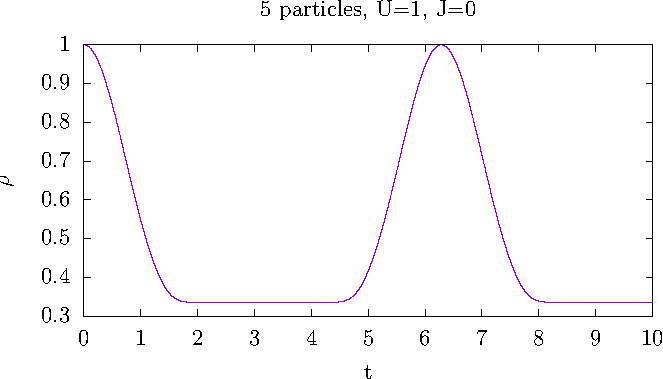
\includegraphics[width=\textwidth]{Figures/TimeEvo5_U1_J0.pdf}
        \caption{\textit{Condensate fraction calculated from a 5 particle, 5 site MPS after performing 10 DMRG sweeps with an SF Hamiltonian ($J=1$, $U=0$) followed by time evolution with a Mott Hamiltonian ($J=0, U=1$).}}
        \label{fig:TimeEvo5_U1_J0}
    \end{subfigure}
    ~
    \begin{subfigure}[t]{0.49\textwidth}
        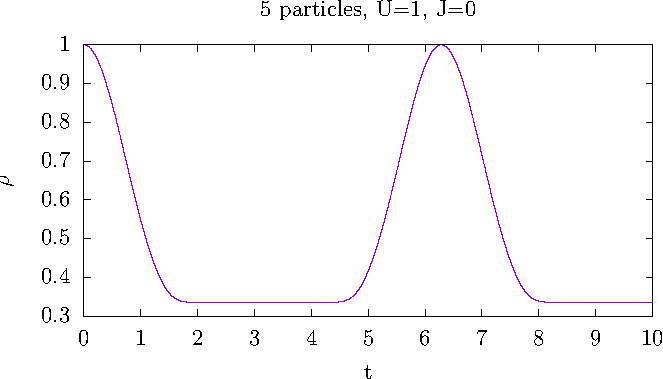
\includegraphics[width=\textwidth]{Figures/TimeEvo50_U1_J0.pdf}
        \caption{\textit{Condensate fraction calculated from a 50 particle, 50 site MPS after performing 20 DMRG sweeps with an SF Hamiltonian ($J=1$, $U=0$) followed by time evolution with a Mott Hamiltonian ($J=0, U=1$).}}
        \label{fig:TimeEvo50_U1_J0}
    \end{subfigure}    
\end{figure}
Figure \ref{fig:TimeEvo5_U1_J0} shows time evolution for 5 particles, whereas \ref{fig:TimeEvo50_U1_J0} is for 50 particles \\(note: figure not yet made)\\ with $U=1$, the period, that is, the time for a full revival of the condensation fraction to occur, can be seen from both figures to be $T=2\pi$. 

WAITING FOR DATA...

\subsection{Time evolution with mixed Hamiltonian}
Performing time evolution on an SF state with a nonzero $J$, the condensate fraction does not achieve full revival, but instead the phases of the individual particle states interfere with each other more and more for each cycle, leading to a decreasing maximal condensate fraction and some spurious lumps in between the peaks, see fig. \ref{fig:TimeEvo5_U2_J0_03}. The period of revival is $T=\pi$, since now $U=2$.

\begin{figure}[h!]
    \centering
    \begin{subfigure}[t]{0.49\textwidth}
        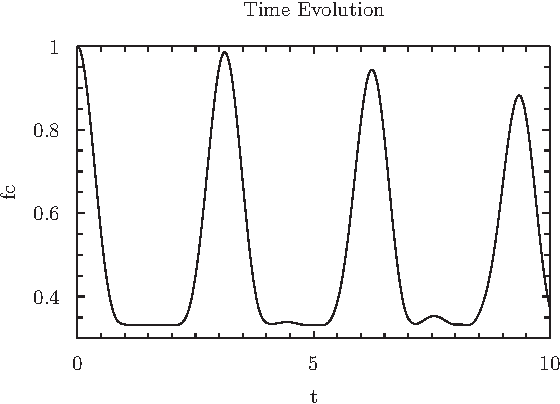
\includegraphics[width=\textwidth]{Figures/TimeEvo5_U2_J0_03.pdf}
        \caption{\textit{Condensate fraction calculated from a 5 particle, 5 site MPS after performing 10 DMRG sweeps with an SF Hamiltonian ($J=1$, $U=0$) followed by time evolution with a ($J=0.03, U=2$) Hamiltonian.}}
        \label{fig:TimeEvo5_U2_J0_03}
    \end{subfigure}
    ~
    \begin{subfigure}[t]{0.49\textwidth}
        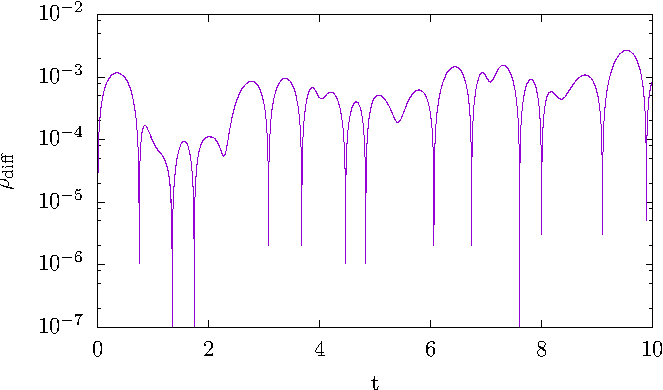
\includegraphics[width=\textwidth]{Figures/TimeEvo5_U2_J0_03_VS_ExactDiag.pdf}
        \caption{\textit{Condensate fraction calculated from a 5 particle, 5 site MPS after performing 10 DMRG sweeps with an SF Hamiltonian ($J=1$, $U=0$) followed by time evolution with a ($J=0.03, U=2$) Hamiltonian compared with the same calculations done with exact diagonalization.}}
        \label{fig:ExDiagComp_U2_J0_03}
    \end{subfigure}
\end{figure}

In fig. \ref{fig:ExDiagComp_U2_J0_03}, the absolute difference between the condensate fraction calculated by MPS formalism and that calculated by exact diagonalization is plotted. The disagreement, while still small at $t=10$, is expected to grow larger for larger times, as the MPS does a series of truncations each time the time evolution MPO is applied to avoid increasing the bond dimension of the MPS, whereas exact diagonalization using the Lanczos algorithm detailed in \cite{Lanczos} is limited mainly by machine precision.